
\changeunitlength{0.035pt}
\def\Compound1{\benzenev{1==O;2==O;3==O}}; 
\def\CompoundA{\benzenev{1==H;}}; 
\def\CompoundB{\sixheteroh{3==O;5==O}};

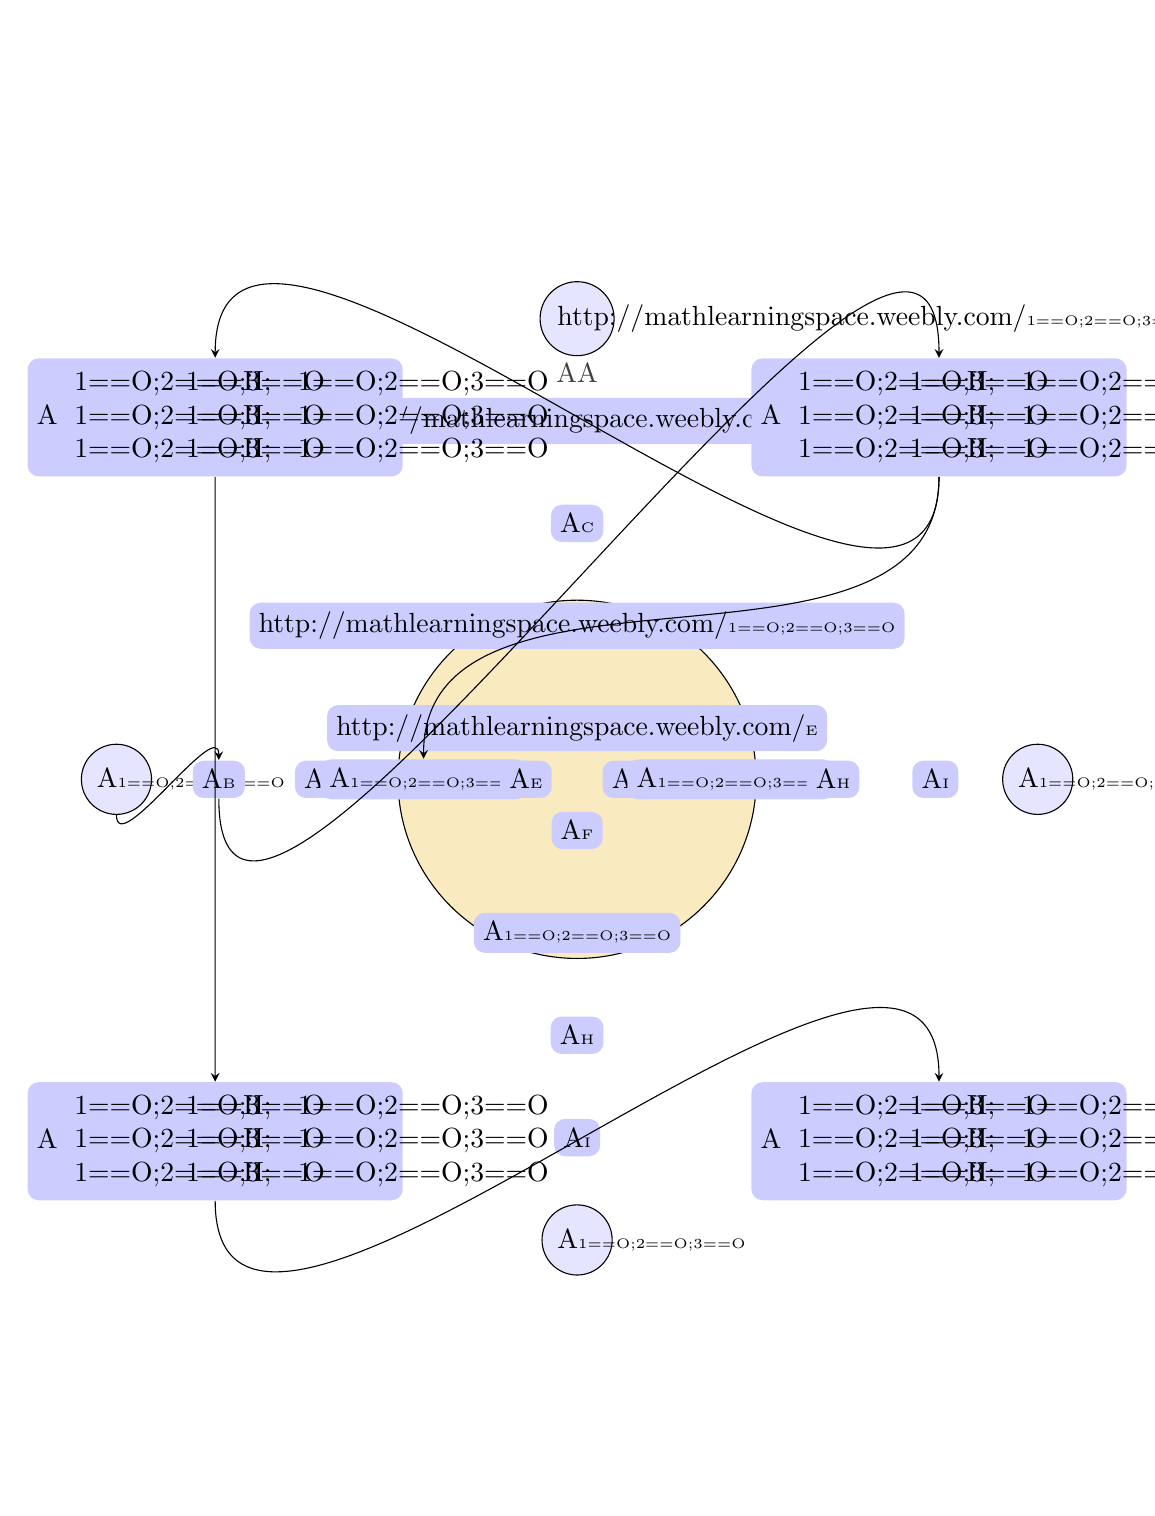
\begin{tikzpicture}[every path/.style = { ->,> = stealth, rounded corners},state/.style = {fill =blue!20,text centered},node distance=1.25cm,scale=0.65]
\centering
\definecolor{color1}{HTML}{E7AD00}
\definecolor{color2}{HTML}{A5CC19}
\definecolor{color3}{HTML}{33B29A}
\definecolor{color4}{HTML}{3380FF}
\definecolor{color5}{HTML}{9033FF}
\definecolor{color6}{HTML}{E5003D}
%--------------------------------------------
\tikzstyle{mbigblock} = [rectangle, draw, text width=2cm, text centered, rounded corners, minimum height=1em]
\tikzstyle{block}  = [circle, draw, text width=0.5cm, fill=blue!10,text centered, minimum height=0.25em]
\tikzstyle{lblock} = [rectangle, draw, text width=2cm,fill=blue!20, text centered, minimum height=1em]
\tikzstyle{rblock} = [rectangle, draw, text width=2cm,fill=red!20, text centered, minimum height=1em]
\tikzstyle{zblock} = [ellipse, draw, text width=2cm,fill=green!30, text centered, minimum height=1em]
\tikzstyle{kblock} = [ellipse, draw, text width=10cm,fill=green!30, text centered, minimum height=1em]
\begin{scope}[opacity = 1,fill opacity = 0.25,text opacity = 0.75,text width = 6em,text centered]
\def\firstcircle{(90:0cm) circle (3.5cm)}
\draw [fill = color1] \firstcircle node [above = 14em] {\href{A}{A}};
\end{scope}
%------------------------------------------------------
\begin{scope}
\node[block] (A) at (90:9) {\href{http://mathlearningspace.weebly.com/}{\tiny{\Compound1}}};
\node[state] (B) at (90:7) {\href{http://mathlearningspace.weebly.com/}{\tiny{B}}};
\node[state] (C) at (90:5) {\href{A}{\tiny{C}}};
%------------------------------------------------------
\node[state] (D) at (90:3) {\href{http://mathlearningspace.weebly.com/}{\tiny{\Compound1}}};
\node[state] (E) at (90:1) {\href{http://mathlearningspace.weebly.com/}{\tiny{E}}};
\node[state] (F) at (90:-1) {\href{A}{\tiny{F}}};
%------------------------------------------------------
\node[state] (G) at (90:-3) {\href{A}{\tiny{\Compound1}}};
\node[state] (H) at (90:-5) {\href{A}{\tiny{H}}};
\node[state] (I) at (90:-7) {\href{A}{\tiny{I}}};
\node[block] (J) at (90:-9) {\href{A}{\tiny{\Compound1}}};
%--------------------------------------------------------
\node[block] (A1) at (180:9) {\href{A}{\tiny{\Compound1}}};
\node[state] (B1) at (180:7) {\href{A}{\tiny{B}}};
\node[state] (C1) at (180:5) {\href{A}{\tiny{C}}};
%---------------------------------------------------------
\node[state] (D1) at (180:3) {\href{A}{\tiny{\Compound1}}};
\node[state] (E1) at (180:1) {\href{A}{\tiny{E}}};
\node[state] (F1) at (180:-1) {\href{A}{\tiny{F}}};
%----------------------------------------------------------
\node[state] (G1) at (180:-3) {\href{A}{\tiny{\Compound1}}};
\node[state] (H1) at (180:-5) {\href{A}{\tiny{H}}};
\node[state] (I1) at (180:-7) {\href{A}{\tiny{I}}};

\node[block] (J) at (180:-9) {\href{A}{\tiny{\Compound1}}};
%----------------------------------
%--------------------------------Anotations-----------------------------------
%----------------------------------
\node[state] (C1) at (45:10)  {\href{A}{\begin{tabular}{p{1cm}p{1cm}p{1cm}}
 \Compound1 & \CompoundA  & \Compound1 \\
 \Compound1 & \CompoundA  & \Compound1 \\
 \Compound1 & \CompoundA  & \Compound1 \\
 \end{tabular}}};
\node[state] (C2) at (135:10) {\href{A}{\begin{tabular}{p{1cm}p{1cm}p{1cm}} 
\Compound1 & \CompoundA  & \Compound1 \\ 
\Compound1 & \CompoundA  & \Compound1 \\
 \Compound1 & \CompoundA  & \Compound1 \\
\end{tabular}}};
\node[state] (C3) at (225:10) {\href{A}{\begin{tabular}{p{1cm}p{1cm}p{1cm}} 
\Compound1 & \CompoundA  & \Compound1 \\ 
\Compound1 & \CompoundA  & \Compound1 \\
\Compound1 & \CompoundA  & \Compound1 \\
\end{tabular}}};
\node[state] (C4) at (315:10) {\href{A}{\begin{tabular}{p{1cm}p{1cm}p{1cm}} 
\Compound1 & \CompoundA  & \Compound1 \\ 
\Compound1 & \CompoundA  & \Compound1 \\
\Compound1 & \CompoundA  & \Compound1 \\
\end{tabular}}}; 
\end{scope}
%-----------------------------------------------------
\path[draw] (C1) edge[out=-90, in=90] (C2);
\path[draw] (C2) edge[out=-90, in=90] (C3);
\path[draw] (C3) edge[out=-90, in=90] (C4);
\path[draw] (A1) edge[out=-90, in=90] (B1);
\path[draw] (B1) edge[out=-90, in=90] (C1);
\path[draw] (C1) edge[out=-90, in=90] (D1);
\end{tikzpicture}%
